\section{Extending Cloud9}
\label{sec:Approaches}
During the development of our sample application \emph{Tetris} we found three major issues that disrupted our development work flow.
We briefly address each of them in this section.

\subsection{Collaboration}
As mentioned in~\ref{sec:tetris} we implemented our sample application in a team of three people.
We expected to use Cloud9 as a collaboration tool.
At the moment we started our project there was no possibilty to add team members to a project on a Cloud9 dashboard.
The collaboration in  was restricted to collaboration with the aid of a git or mercurial repository.
Thus using a repository as we were used to beforehand was the only way of having collaboration.

Actually we wanted to be able to see what other team members do during development, e.g.:
\begin{packed_itemize}
    \item Is another team member working on the same project as well?
    \item At what file is the team member working?
    \item At what exactly does the team member is working at?
\end{packed_itemize}
Moreover we wanted to be able to communicate with one another.
Since all this was not supported by Cloud9 this was one extension we planned to implement.

\subsection{IDE-based Issue-Tracking}
Not only during the development of our sample application but also during our every day development would we like to be supported by automatic issue tracking.
Thus we want to extend Cloud9 to handle automatic issue tracking.
For this extension two different aspects were important for us.
On one hand we wanted to know how long we've worked on which file.
So this extension would have to track the focus time of files and, if possible, in a more fine-grained level what methods or the like were edited in the file.
On the other hand we wanted automatic issue creation.
For that we wanted to recognize if the developer annotated any code with e.g. \texttt{TODO}, \texttt{FIXME} or \texttt{BUG} and automatically create issues.
Therefore this extension would include an issue tracker for Cloud9.
If the project is linked to a GitHub or bitbucket repository the respective issue tracking API of either of them should be used to create corresponding issues there as well.

\subsection{Appropriate git integration}
\label{subsec:ext_git_integration}
As we stated in~\ref{sec:tetris} two of us already knew git and developed several projects using git.
Both are used to use the console to execute git commands. Only for going through the repository history or branches they prefer a graphical tool.
Therefore it was not surprising that developers have to use the console in Cloud9 as well.
Unfortunately the Cloud9 client console is not powerful enough to support the git workflow we are used to.
Neither \texttt{git status} nor \texttt{git diff} is displayed in color.
Therefore it is very hard to get information from the console output as shown in figure~\ref{fig:diff_output}.
Furthermore the console is not interactive which includes that large output (from e.g. \texttt{git diff}) will be displayed at once glutting developers and \texttt{git add --patch} is not even working.
Developers use this command to seperate semantically different changes within files into different commits.

One of us has not used git before.
So the whole process of using git was not familiar to him.
He had to learn all the git commands and got no help from Cloud9.
With the non-colored output it is even harder to understand the mechanics of git.
For git beginners it would be easier to get familiar with git if they got support from their development environment.
As for a Cloud9 extension we want to extend the user interface: 
Visual controls should enable the execution of common git commands.
Additionally git diff output should be visualized with color and immediately.

In sum the extension should integrate a proper git workflow and facilitate first steps into git.
To further improve the development workflow we want to avoid switching back and forth between code editor and console completely.
Additionally we want to track code changes and visualize them while development in the editor.

\begin{figure}
   \centering
   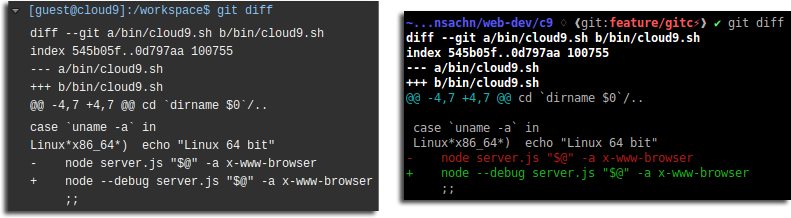
\includegraphics[width=0.9\textwidth]{images/diff_output.png}
   \caption{On both consoles is a part of a \texttt{git diff} command output.
   The left side shows the Cloud9 console and the right side shows a unix bash console.
   The \texttt{+} and \texttt{-} at the beginning of a line inidcate either added or deleted lines.
   But with the aid of color it is much easier to find information in that output, especially when there are many changes.}
   \label{fig:diff_output}
\end{figure}


\subsection{Our choice}
The collaboration extension of Cloud9 is already in development and is to be released in about 3 weeks.
We hope to develop an extension that might be integrated into the main Cloud9 project.
Because of that we chose not to implement yet another collaboration extension.

We feel that proper repository integration is needed in almost all projects e.g. due to the need of history and backups.
Whereas there might be less projects needing issue-tracking e.g. a very small project.
That is why we chose to implement an extension that enables Cloud9 to support users with proper git integration and helps git beginners to get started with git.

